\documentclass[12pt]{report}
\usepackage[utf8]{inputenc}
\usepackage[russian]{babel}
%\usepackage[14pt]{extsizes}
\usepackage{listings}
\usepackage{graphicx}
\usepackage{amsmath,amsfonts,amssymb,amsthm,mathtools} 
\usepackage{pgfplots}
\usepackage{filecontents}
\usepackage{indentfirst}
\usepackage{eucal}
\usepackage{float} 
\usepackage{amsmath}
\usepackage{enumitem}
\usepackage[justification=centering]{caption} 
\usepackage{tikz}
\usepackage{pgfplots}
\pgfplotsset{compat=newest}

\frenchspacing

\usepackage{indentfirst} % Красная строка


%\usetikzlibrary{datavisualization}
%\usetikzlibrary{datavisualization.formats.functions}

\usepackage{amsmath}


% Для листинга кода:
\lstset{ %
language=haskell,                 % выбор языка для подсветки (здесь это С)
basicstyle=\small\sffamily, % размер и начертание шрифта для подсветки кода
numbers=left,               % где поставить нумерацию строк (слева\справа)
numberstyle=\tiny,           % размер шрифта для номеров строк
stepnumber=1,                   % размер шага между двумя номерами строк
numbersep=5pt,                % как далеко отстоят номера строк от подсвечиваемого кода
showspaces=false,            % показывать или нет пробелы специальными отступами
showstringspaces=false,      % показывать или нет пробелы в строках
showtabs=false,             % показывать или нет табуляцию в строках
frame=single,              % рисовать рамку вокруг кода
tabsize=2,                 % размер табуляции по умолчанию равен 2 пробелам
captionpos=t,              % позиция заголовка вверху [t] или внизу [b] 
breaklines=true,           % автоматически переносить строки (да\нет)
breakatwhitespace=false, % переносить строки только если есть пробел
escapeinside={\#*}{*)}   % если нужно добавить комментарии в коде
}

\usepackage[left=2cm,right=2cm, top=2cm,bottom=2cm,bindingoffset=0cm]{geometry}
% Для измененных титулов глав:
\usepackage{titlesec, blindtext, color} % подключаем нужные пакеты
\definecolor{gray75}{gray}{0.75} % определяем цвет
\newcommand{\hsp}{\hspace{20pt}} % длина линии в 20pt
% titleformat определяет стиль
\titleformat{\chapter}[hang]{\Huge\bfseries}{\thechapter\hsp\textcolor{gray75}{|}\hsp}{0pt}{\Huge\bfseries}


% plot
\usepackage{pgfplots}
\usepackage{filecontents}
\usetikzlibrary{datavisualization}
\usetikzlibrary{datavisualization.formats.functions}

\begin{document}
%\def\chaptername{} % убирает "Глава"
\thispagestyle{empty}
\begin{titlepage}
	\noindent \begin{minipage}{0.15\textwidth}
	
\includegraphics[width=\linewidth]{b_logo}
	\end{minipage}
	\noindent\begin{minipage}{0.9\textwidth}\centering
		\textbf{Министерство науки и высшего образования Российской Федерации}\\
		\textbf{Федеральное государственное бюджетное образовательное учреждение высшего образования}\\
		\textbf{~~~«Московский государственный технический университет имени Н.Э.~Баумана}\\
		\textbf{(национальный исследовательский университет)»}\\
		\textbf{(МГТУ им. Н.Э.~Баумана)}
	\end{minipage}
	
	\noindent\rule{18cm}{3pt}
	\newline\newline
	\noindent ФАКУЛЬТЕТ $\underline{\text{«Информатика и системы управления»}}$ \newline\newline
	\noindent КАФЕДРА $\underline{\text{«Программное обеспечение ЭВМ и информационные технологии»}}$\newline\newline\newline\newline\newline
	
	
	\begin{center}
		\noindent\begin{minipage}{1.3\textwidth}\centering
			\Large\textbf{  Отчёт по лабораторной работе №5}\newline
			\textbf{по дисциплине "Анализ алгоритмов"}\newline\newline
		\end{minipage}
	\end{center}
	
	\noindent\textbf{Тема} $\underline{\text{Конвейерные вычисления}}$\newline\newline
	\noindent\textbf{Студент} $\underline{\text{Варламова Е. А.}}$\newline\newline
	\noindent\textbf{Группа} $\underline{\text{ИУ7-51Б}}$\newline\newline
	\noindent\textbf{Преподаватели} $\underline{\text{Волкова Л.Л.}}$\newline\newline\newline
	
	\begin{center}
		\vfill
		Москва~---~\the\year
		~г.
	\end{center}
\end{titlepage}

\setcounter{page}{2}
\tableofcontents

\newpage
\chapter*{Введение}
\addcontentsline{toc}{chapter}{Введение}

При обработке данных могут возникать ситуации, когда один набор данных необходимо обработать последовательно несколькими алгоритмами. В таком случае удобно использовать идею конвейерной обработки. Конвейер - механизм организации труда, при котором производство изделия разбивается на стадии, и конкретные работники закрепляются за своими стадиями. Таким образом, обработка делится на линии конвейера. При этом каждая следующая линия обрабатывает данные только тогда, когда предыдущая завершила свою работу над теми же данными. 

Здесь также можно заметить, что обработка данных на разных линиях конвейера может быть выполнена параллельно, что значительно улучшит производительность конвейра за счёт уменьшения времени простоя линий.

Целью данной работы является  изучение и реализация параллельной и линейной реализаций конвейерной обработки данных. Для достижения поставленной цели необходимо решить следующие задачи:
\begin{itemize}
    \item изучить конвейерную обработку данных;
    \item разработать метод конвейерной обработки данных на примере приготовления печенья;
	\item реализовать систему конвейерных вычислений;
	\item сравнить параллельную и последовательную реализации конвейерных вычислений на основе собранной статистики.
\end{itemize}

\chapter{Аналитическая часть}

В данном разделе представлены теоретические сведения о рассматриваемых алгоритмах.

\section{Конвейерная обработка данных}

Конвейер - это механизм, который позволяет обрабатывать однотипные заявки поэтапно. Поэтому конвейер представляет собой некоторое количество лент, на каждой из которых выполняется одинаковая работа над поступающими заявками. В терминах программирования ленты конвейера представлены функциями-обработчиками, выполняющими над неким набором данных операции и передающими их на следующую ленту конвейера. Очевидно, что моделирование конвейерной обработки хорошо сочетается с технологией многопоточного программирования, так как под каждую ленту конвейера может быть выделен отдельный поток. 

\section{Описание задачи}

Для моделирования системы конвейерной обработки данных был выбран процесс приготовления печенья в производственных масштабах, состоящий из трех этапов:

\begin{itemize}
	\item подсчёт массы куриных яиц в мг (вычисление n-ого числа Фибоначчи);
	\item подсчёт массы масла в мг (возведение в степень)
	\item подсчёт массы муки в мг (факториал числа).
\end{itemize}

\section*{Вывод}
В данном разделе были рассмотренны особенности построения конвейерных вычислений.

\chapter{Конструкторская часть}

В данном разделе представлены схемы рассматриваемых алгоритмов.

\section{Разработка алгоритмов}

На рисунке \ref{fig:com} приведена общая схема организации конвейерных вычислений для каждой заявки. 

\begin{figure}[h]
	\centering
	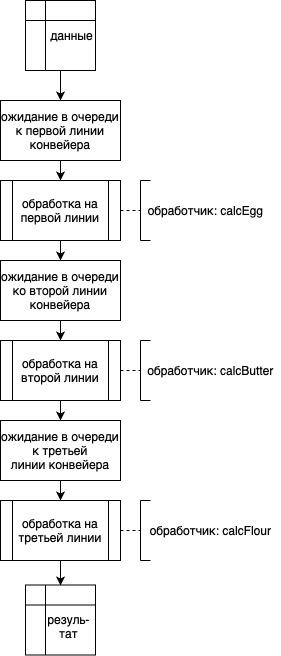
\includegraphics[scale = 0.6]{common.jpg}
	\caption{Общая схема организации конвейерных вычислений.}
	\label{fig:com}
\end{figure}
\newpage

На рисунке \ref{mainThread} приведена схема главного потока для параллельной обработки заявок.

\begin{figure}[h]
	\centering
	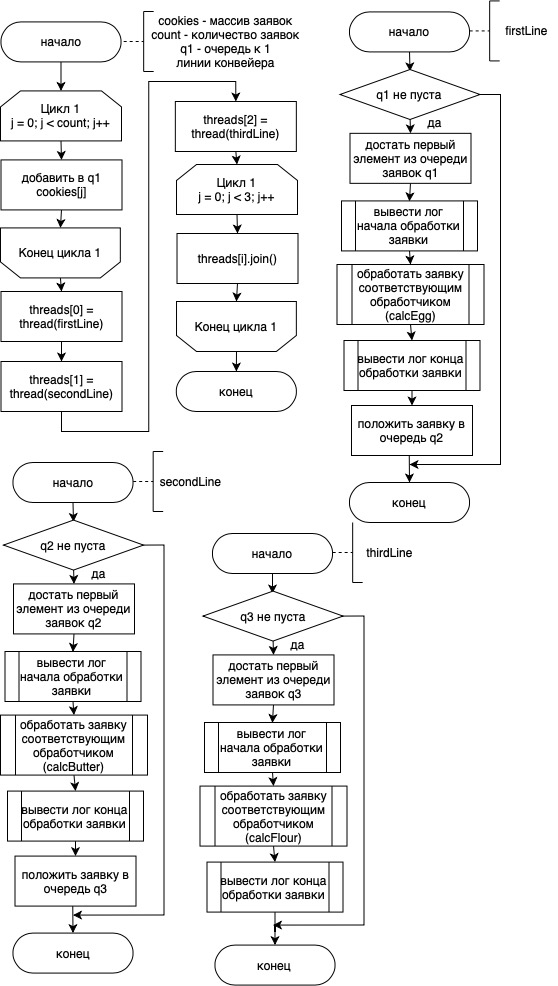
\includegraphics[scale = 0.51]{mainThread.jpg}
	\caption{Схема главного потока для параллельной обработки заявок}
	\label{mainThread}
\end{figure}

\newpage

На рисунке \ref{fig:steps} приведены схемы каждого типа вычислений конвейера. 
\begin{figure}[h]
	\centering
	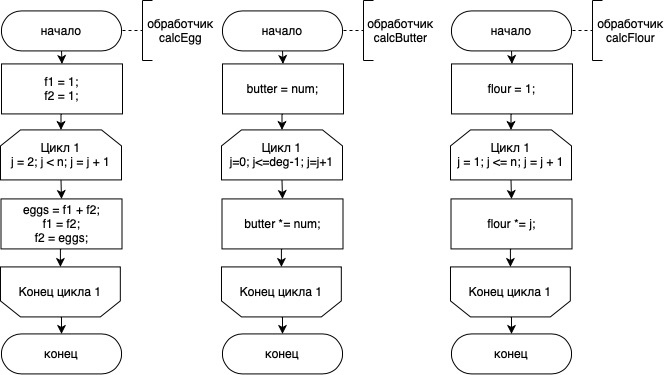
\includegraphics[width = \linewidth]{steps.jpg}
	\caption{Схемы трёх типов вычислений конвейера}
	\label{fig:steps}
\end{figure}

\section{Используемые структуры данных}
Для организации потокобезопасных очередей было решено использовать обёртку над стандартным типом данных очередь. Такая очередь обеспечивает монопольное владение ресурсом каждым потоком, что не позволяет привести к ситуации гонки. Так, каждый вызов методов очереди блокируется мьютексом.
\section*{Вывод}
На основе анализа принципа работы конвейера была разработана общая схема организации конвейерных вычислений и схемы вычислений на каждой ленте конвейера в соответствии с выбранным для моделирования процессом. Кроме того, были выбраны используемые структуры данных.

\chapter{Технологическая часть}

В данном разделе приведены средства реализации и листинги кода.

\section{Средства реализации}
Для реализации был выбран язык программирования C++. Данный выбор обусловлен наличием инструментов для создания и эффективной работы с потоками. В качестве среды разработки была выбрана среда CLion. 

\section{Реализация алгоритмов}

В листингах \ref{linCode} и \ref{parCode} приведены однопоточная и многопоточная реализации конвейерных вычислений, в листинге \ref{queueCode} - реализация потокобезопасной очереди, а в листинге \ref{stepsCode} - реализация обработчиков, представляющих этапы конвейера.
\begin{lstlisting}[label=linCode,caption=Однопоточная реализация конвейера,language=C]
void Conveyor::run_seq(size_t count) {
    for (size_t i = 0; i < count; i++) {
        std::shared_ptr<Сookies> c(new Cookies);
        c->calcEgg(1000000);
        c->calcButter(2, 1000000);
        c->calcFlour(1000000);
    }
}
\end{lstlisting}

\begin{lstlisting}[label=parCode,caption=Многопоточная реализация конвейера ,language=C]
void Conveyor::run_par(size_t count) {
    for (size_t i = 0; i < count; i++) {
        std::shared_ptr<Сookies> p(new Cookies);
        cookies.push_back(p);
        q1.push(p);
    }
    this->threads[0] = std::thread(&Conveyor::calcEgg, this);
    this->threads[1] = std::thread(&Conveyor::calcButter, this);
    this->threads[2] = std::thread(&Conveyor::calcFlour, this);
    for (int i = 0; i < 3; i++) {
        this->threads[i].join();
    }
}
void Conveyor::calcEgg()
{
    size_t task_num = 1;
    while (!this->q1.empty()) {
        std::shared_ptr<Cookies> c = q1.front();
        log_current_event(task_num, "Part 1 | Start");
        c->calcEgg(1000000);
        log_current_event(task_num, "Part 1 | End");
        q2.push(c);
        q1.pop();
        task_num++;
    }

}
void Conveyor::calcButter()
{
    size_t task_num = 1;
    do {
        if (!this->q2.empty()) {
            std::shared_ptr<Cookies> c = q2.front();
            log_current_event(task_num, "Part 2 | Start");
            c->calcButter(2, 1000000);
            log_current_event(task_num, "Part 2 | End");
            q3.push(c);
            q2.pop();
            task_num++;
        }
    } while(!q1.empty() || !q2.empty());
}
void Conveyor::calcFlour()
{
    size_t task_num = 1;
    do {
        if (!this->q3.empty()) {
            std::shared_ptr<Cookies> c = q3.front();
            log_current_event(task_num, "Part 3 | Start");
            c->calcFlour(1000000);
            log_current_event(task_num, "Part 3 | End");
            q3.pop();
            task_num++;
        }
    } while (!q1.empty() || !q2.empty() || !q3.empty());
}
\end{lstlisting}
\newpage
\begin{lstlisting}[label=queueCode,caption=Реализация потокобезопасной очереди,language=C]
std::mutex mtx;
template <typename type>
void SafeQueue<type>::push(type val)
{
    mtx.lock();
    q.push(val);
    mtx.unlock();
}
template <typename type>
void SafeQueue<type>::pop()
{
    mtx.lock();
    q.pop();
    mtx.unlock();
}
template <typename type>
bool SafeQueue<type>::empty()
{
    bool r;
    mtx.lock();
    r = q.empty();
    mtx.unlock();
    return r;
}
template <typename type>
type SafeQueue<type>::front()
{
    type val;
    mtx.lock();
    val = q.front();
    mtx.unlock();
    return val;
}
\end{lstlisting}
\newpage
\begin{lstlisting}[label=stepsCode,caption=Обработчики линий конвейера,language=C]
void Cookies::calcEgg(int n) // fib
{
    int f1 = 1, f2 = 1;

    for (int i = 2; i < n; i++)
    {
        this->eggs = f1 + f2;
        f1 = f2;
        f2 = this->eggs;
    }
}
void Cookies::calcButter(int num, int deg)  // num ^ degree
{
    this->butter = num;
    for (int i = 0; i < deg - 1; i++)
        this->butter *= num;
}
void Cookies::calcFlour(long n)  // factorial
{
    this->flour = 1;
    for (int i = 1; i <= n; i++)
        this->flour *= i;
}
\end{lstlisting}


\section*{Вывод}

В данном разделе была реализована конвейерная обработка данных на примере моделировани процесса приготовления печенья, кроме того, были выбраны средства разработки.

\chapter{Исследовательская часть}

В данном разделе приведен анализ характеристик разработанного ПО  и примеры работы ПО.

\section{Технические характеристики ЭВМ}

Все нижепреведенные замеры времени проведены на процессоре: Intel Core i5, 1,4 GHz, четырёхъядерный, количество логических ядер - 8. Время работы алгоритмов было замерено с помощью chrono [1].

\section{Время выполнения алгоритмов}

На рисунке \ref{cmp} приведено сравнение времени выполнения параллельной и последовательной обработки данных в зависимости от количества входных задач. При этом предполгаается, что на лентах конвейера заявки обрабатываются примерно за одинаковое время. В таблице \ref{tableComp} приведена статистика выполнения заявок в зависимости от количества заявок: указано среднее время выполнения заявки (время, которое заявка занимала у всех линий конвейера), среднее время ожидания в очереди и среднее время пребывания в системе. В листинге \ref{queueTasks} приведён лог параллельной обработки восьми заявок.

\begin{table} [h!]
	\caption{Таблица времени выполнения параллельной обработки данных (в мс)}
	\label{tableComp}
	\begin{center}
		\begin{tabular}{|c c c c|} 
		 	\hline
			Количество задач & t в очереди & t в системе & t обработки \\  
			\hline
            100 & 213.990 & 224.430 & 10.440 \\
            \hline
            200 & 442.710 & 453.185 & 10.475 \\
            \hline
            300 & 667.347 & 677.813 & 10.467 \\
            \hline
            400 & 907.885 & 918.395 & 10.510 \\
            \hline
            500 & 957.998 & 967.982 & 9.984 \\
            \hline
            600 & 1370.842 & 1381.335 & 10.493 \\
            \hline
            700 & 1587.126 & 1597.559 & 10.433 \\
            \hline
            800 & 1802.399 & 1812.965 & 10.566 \\
            \hline
            900 & 2022.898 & 2033.367 & 10.469 \\
            \hline
            1000 & 2275.780 & 2286.326 & 10.546 \\
			\hline
		\end{tabular}
	\end{center}
\end{table}
\newpage
\begin{lstlisting}[label=queueTasks,caption=Лог параллельной обработки восьми заявок,language=C]
Task №1 | Part 1 | Start | 13:09:10.629
Task №1 | Part 1 | End | 13:09:10.855
Task №2 | Part 1 | Start | 13:09:10.855
Task №1 | Part 2 | Start | 13:09:10.855
Task №1 | Part 2 | End | 13:09:11. 27
Task №1 | Part 3 | Start | 13:09:11. 27
Task №2 | Part 1 | End | 13:09:11. 80
Task №3 | Part 1 | Start | 13:09:11. 80
Task №2 | Part 2 | Start | 13:09:11. 80
Task №1 | Part 3 | End | 13:09:11.200
Task №2 | Part 2 | End | 13:09:11.253
Task №2 | Part 3 | Start | 13:09:11.253
Task №3 | Part 1 | End | 13:09:11.307
Task №4 | Part 1 | Start | 13:09:11.307
Task №3 | Part 2 | Start | 13:09:11.307
Task №2 | Part 3 | End | 13:09:11.426
Task №3 | Part 2 | End | 13:09:11.480
Task №3 | Part 3 | Start | 13:09:11.480
Task №4 | Part 1 | End | 13:09:11.532
Task №5 | Part 1 | Start | 13:09:11.532
Task №4 | Part 2 | Start | 13:09:11.532
Task №3 | Part 3 | End | 13:09:11.652
Task №4 | Part 2 | End | 13:09:11.704
Task №4 | Part 3 | Start | 13:09:11.704
Task №5 | Part 1 | End | 13:09:11.758
Task №6 | Part 1 | Start | 13:09:11.758
Task №5 | Part 2 | Start | 13:09:11.758
Task №4 | Part 3 | End | 13:09:11.878
Task №5 | Part 2 | End | 13:09:11.931
Task №5 | Part 3 | Start | 13:09:11.931
Task №6 | Part 1 | End | 13:09:11.986
Task №7 | Part 1 | Start | 13:09:11.986
Task №6 | Part 2 | Start | 13:09:11.986
Task №5 | Part 3 | End | 13:09:12.107
Task №6 | Part 2 | End | 13:09:12.161
Task №6 | Part 3 | Start | 13:09:12.161
Task №7 | Part 1 | End | 13:09:12.217
Task №8 | Part 1 | Start | 13:09:12.217
Task №7 | Part 2 | Start | 13:09:12.217
Task №6 | Part 3 | End | 13:09:12.338
Task №7 | Part 2 | End | 13:09:12.393
Task №7 | Part 3 | Start | 13:09:12.393
Task №8 | Part 1 | End | 13:09:12.449
Task №8 | Part 2 | Start | 13:09:12.449
Task №7 | Part 3 | End | 13:09:12.566
Task №8 | Part 2 | End | 13:09:12.621
Task №8 | Part 3 | Start | 13:09:12.621
Task №8 | Part 3 | End | 13:09:12.793
\end{lstlisting}
\newpage
\begin{figure}[h]
	\centering
	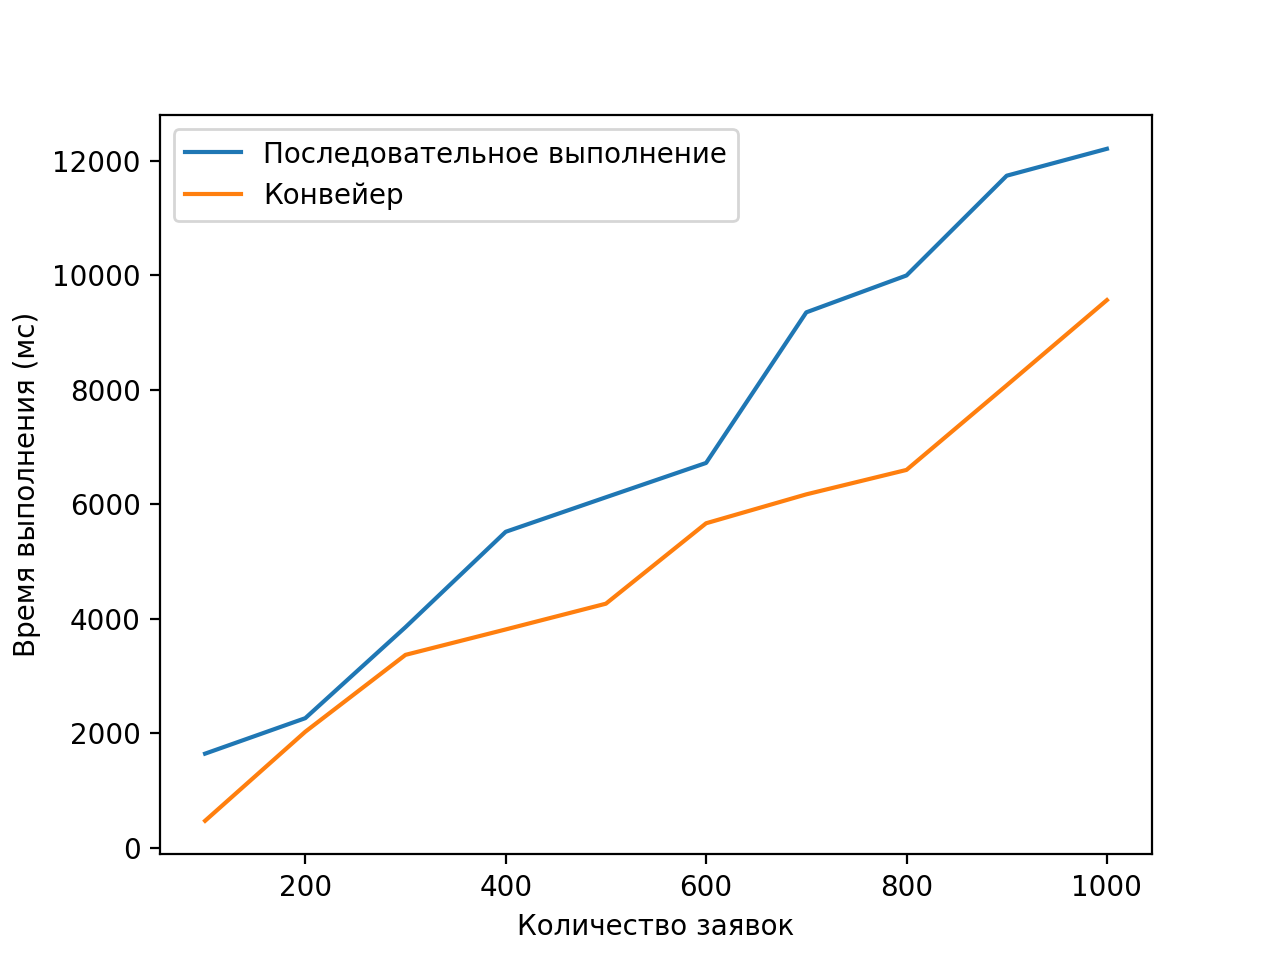
\includegraphics[width = \linewidth]{cmp.png}
	\caption{Cравнение времени выполнения параллельной и последовательной обработки данных (в мс).}
	\label{cmp}
\end{figure}
\section*{Вывод}

В результате исследования было выяснено, что многопотчная реализация конвейера работает быстрее, чем линейная. Кроме того, с увеличением количества заявок растёт и время ожидания в очереди к линиям конвейера.
\chapter*{Заключение}
\addcontentsline{toc}{chapter}{Заключение}

В рамках данной лабораторной работы были решены следующие задачи:
\begin{itemize}
    \item изучена конвейерная обработка данных;
    \item разработан метод конвейерной обработки данных на примере приготовления печенья;
	\item реализована система конвейерных вычислений;
	\item было проведено сравнение параллельной и линейной реализаций конвейерных вычислений на основе собранной статистики.
\end{itemize}

Параллельные конвейерные вычисления позволяют организовать непрерывную обработку данных, что позволяет выиграть время в задачах, где требуется обработка больших объемов данных за малый промежуток времени.

Поставленная цель была достигнута.


\chapter*{Литература}
\addcontentsline{toc}{chapter}{Литература}
\begin{enumerate}
	\item Стандартный набор функций для получения значения времени [Электронный ресурс]. Режим доступа: https://en.cppreference.com/w/cpp/chrono. Дата обращения: 16.11.2021
	
\end{enumerate}

\end{document}